% !TEX program = xelatex
% XeLaTeX source for the 5 x 8 inch edition.
\documentclass[10pt,twoside,openany]{book}

\usepackage{geometry}
\geometry{
  paperwidth=5in,
  paperheight=8in,
  top=0.7in,
  bottom=0.7in,
  inner=0.5in,
  outer=0.5in,
  headheight=10pt,
  headsep=20pt,
  footskip=25.2pt
}
\addtolength{\textheight}{-12pt}

\usepackage{fontspec}
\usepackage{xeCJK}
\usepackage{setspace}
\defaultfontfeatures{Ligatures=TeX}
\setmainfont[Path=../fonts/]{SourceHanSerifCN-Regular.otf}
\setCJKmainfont[Path=../fonts/]{SourceHanSerifCN-Regular.otf}
\setsansfont[Path=../fonts/]{SourceHanSansCN-Medium.otf}
\setCJKsansfont[Path=../fonts/]{SourceHanSansCN-Medium.otf}
\newfontfamily\SeparatorFont{lmroman10-regular.otf}
\xeCJKsetup{PunctStyle=plain}

\usepackage{fancyhdr}
\usepackage{xcolor}
\usepackage{pdfpages}
\usepackage[unicode=true,hidelinks]{hyperref}
\definecolor{PrimaryInk}{HTML}{161618}
\definecolor{SecondaryInk}{HTML}{5C5C62}
\color{PrimaryInk}
\hypersetup{
  pdftitle={Ma petite amie Jing Tian},
  pdfauthor={Justin Sun},
  pdfsubject={5 x 8 inch XeLaTeX edition}
}

% Body paragraphs begin flush with the text block.
\setlength{\parindent}{0pt}
\setlength{\parskip}{0pt}
\setlength{\topskip}{10pt}
\renewcommand{\baselinestretch}{1}
\clubpenalty=10000
\widowpenalty=10000
\displaywidowpenalty=10000
\brokenpenalty=10000
\raggedbottom

\fancypagestyle{bodyrunning}{
  \fancyhf{}
  \fancyhead[LO]{\sffamily\fontsize{8}{10}\selectfont\color{SecondaryInk}Ma petite amie Jing Tian}
  \fancyhead[RO]{\sffamily\fontsize{8}{10}\selectfont\color{SecondaryInk}\thepage}
  \fancyhead[LE]{\sffamily\fontsize{8}{10}\selectfont\color{SecondaryInk}\thepage}
  \fancyhead[RE]{\sffamily\fontsize{8}{10}\selectfont\color{SecondaryInk}Ma petite amie Jing Tian}
  \renewcommand{\headrulewidth}{0pt}
  \renewcommand{\footrulewidth}{0pt}
}

\fancypagestyle{bodyopening}{
  \fancyhf{}
  \fancyfoot[C]{\sffamily\fontsize{8}{10}\selectfont\color{SecondaryInk}\thepage}
  \renewcommand{\headrulewidth}{0pt}
  \renewcommand{\footrulewidth}{0pt}
}

\newcommand{\BodySingleLeading}{17.3076923}
\newcommand{\StoryParagraph}[2]{%
  \begingroup
  \rmfamily
  \setstretch{1.3}%
  \fontsize{9.5}{\BodySingleLeading}\selectfont
  #2\par
  \vspace{#1pt}
  \endgroup
}

\newcommand{\NarrativeBreak}{%
  \par\penalty10000
  \vspace{37.4pt}
  \noindent\hbox to \textwidth{\hfil\SeparatorFont\setstretch{1.3}\fontsize{9.5}{\BodySingleLeading}\selectfont\char"002D\kern0.12em\char"002D\kern0.12em\char"002D\hfil}\par
  \vspace{31.4pt}
  \penalty10000
}

\newcommand{\UnprintedPause}{%
  \par\penalty10000\vspace{22pt}\penalty10000
}

\begin{document}
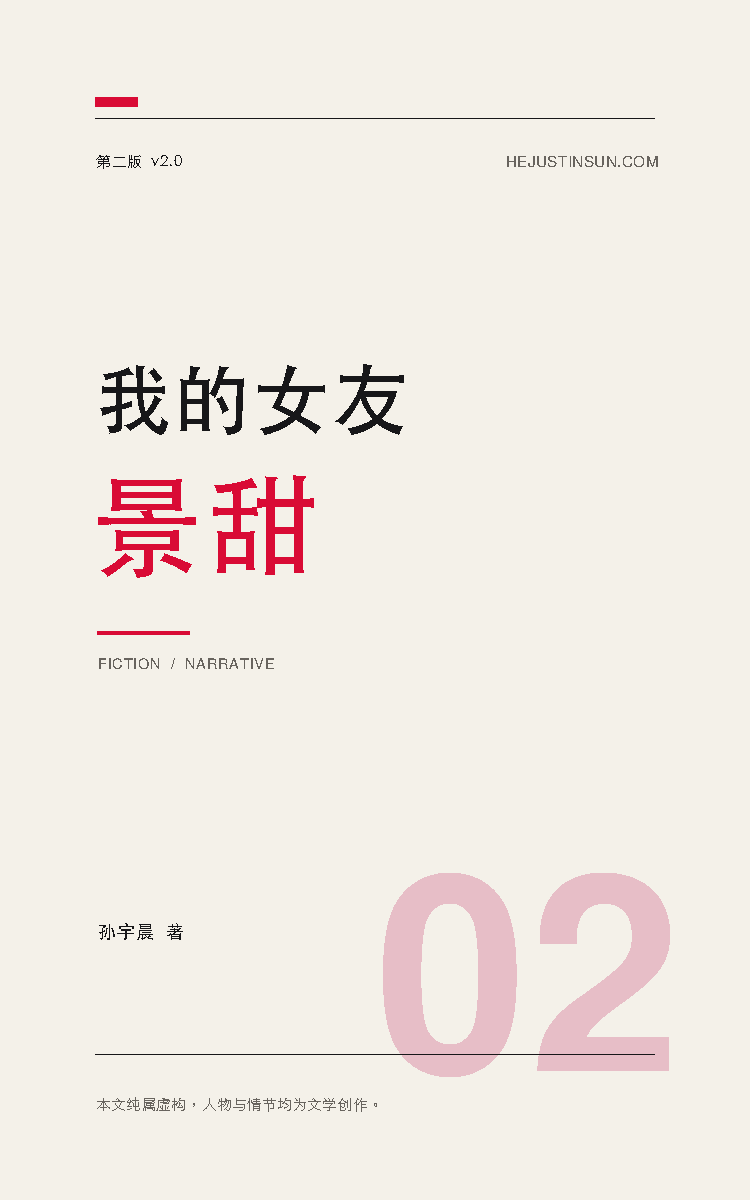
\includepdf[
  pages=1,
  fitpaper=true,
  noautoscale=true,
  pagecommand={\thispagestyle{empty}}
]{../assets/cover.pdf}

\pagenumbering{arabic}
\setcounter{page}{1}
\pagestyle{bodyrunning}
\thispagestyle{bodyopening}
% Opening-page breathing room.
\vspace*{70.817pt}

\StoryParagraph{3}{Le poids d'un ovule : trois microgrammes et demi.}

\StoryParagraph{3}{Le poids de cinquante millions de dollars en liquide : deux tonnes et demie.}

\StoryParagraph{3}{Au téléphone, depuis le Montage Laguna Beach, Jing Tian me demandait le second. Elle mettait le premier en gage.}

\StoryParagraph{3}{Elle était allée là-bas pour la ponction d'ovocytes. L'enfant, porté par une mère porteuse, devait naître en 2027 ; en faisant vite, il serait encore du signe du Cheval. C'était elle qui l'avait proposé. Arrivée à la clinique, elle a dit : pas de cinquante millions, pas de ponction.}

\UnprintedPause

\StoryParagraph{0}{Le Montage Laguna Beach est posé sur la falaise, avec le Pacifique en dessous. L'étage entier, privatisé trente jours, un million de dollars, pour sa tranquillité. Elle y est restée huit jours, puis elle est partie.}

\StoryParagraph{0}{Les vingt-deux jours restants, les femmes de chambre ont continué de monter chaque matin. C'est mon assistante qui me l'a raconté ; en allant rendre les clés, elle en a croisé une : une Mexicaine poussant son chariot, entrant chambre après chambre, changeant les serviettes, essuyant les surfaces, bordant les couvertures, ressortant en refermant la porte. L'étage entier, deux heures.}

\StoryParagraph{0}{Mon assistante lui a demandé pourquoi elle faisait tout ça, puisque personne n'y logeait.}

\StoryParagraph{0}{Elle a dit : sur le registre, c'est occupé.}

\StoryParagraph{0}{Un Versailles qui a perdu sa reine.}

\StoryParagraph{0}{J'ai compris d'un coup : Jing Tian aime ça. Jing Tian aime qu'un lieu reste vide à cause d'elle. Il ne se passe rien.}

\StoryParagraph{3}{Vide avec le Montage Laguna Beach, il y avait aussi un Gulfstream G700, gauchement immobilisé à Van Nuys, l'équipage pointant chaque jour comme d'habitude.}

\StoryParagraph{3}{Le huitième jour, elle a passé ce coup de téléphone. Après, personne ne l'a plus revue.}

\NarrativeBreak

\StoryParagraph{0}{En 2007, quelqu'un brûlait déjà de l'argent pour elle. Cette année-là, j'entrais à Beida.}

\StoryParagraph{3}{Celui qui brûlait l'argent, bien sûr, ce n'était pas moi.}

\StoryParagraph{3}{QQ a fait surgir une fenêtre : l'égérie, c'était elle. Sur ce vieux Lenovo IBM, la résolution était toute floue. J'ai enregistré l'image.}

\StoryParagraph{3}{Depuis mon dortoir de Beida à mille yuans de loyer par an, je l'ai trouvée sur Xiaonei, le Facebook chinois, et j'ai envoyé une demande d'ami. Xiaonei demandait un mot d'accompagnement. J'ai écrit, effacé, réécrit, pendant à peu près quarante minutes ; à la fin je n'ai envoyé qu'un «~Bonjour~».}

\StoryParagraph{3}{Elle n'a pas accepté.}

\StoryParagraph{3}{Peut-être qu'elle n'avait jamais utilisé Xiaonei.}

\StoryParagraph{3}{Toutes ces années, quoi que je fasse, je me posais la même question : à partir de quel niveau accepterait-elle. Au premier milliard, j'y ai pensé. À dix milliards, j'y ai pensé.}

\StoryParagraph{3}{Puis j'ai arrêté d'y penser. Renren avait fermé depuis longtemps.}

\StoryParagraph{3}{Je n'ai jamais refait de demande.}

\StoryParagraph{3}{En 2011, il faisait froid à Pékin. J'ai acheté une doudoune, cent cinquante yuans. Je me souviens du prix, parce que j'ai hésité trois jours.}

\StoryParagraph{3}{La même année, elle tournait Les Royaumes combattants, un film à cent cinquante millions de yuans. Sun Honglei, Francis Ng, Kim Hee-sun, Kiichi Nakai, Jiang Wu avaient été conviés en figurants, comme le seraient dix-neuf ans plus tard le Montage Laguna Beach et le Gulfstream G700 ; ils ne savaient pas ce qu'ils faisaient là, mais puisqu'ils étaient venus, il fallait bien qu'il se passe quelque chose. Il ne s'est rien passé.}

\StoryParagraph{3}{Plus tard, ce fut La Grande Muraille, cent cinquante millions de dollars. Zhang Yimou, Andy Lau, Matt Damon. Plus tard encore, Jackie Chan. La liste de l'univers Jing Tian s'allongeait.}

\StoryParagraph{3}{J'étais déjà en Amérique, les études, les start-up, de plus en plus occupé. Une seule chose n'a pas changé : à chaque nouvel appareil, quelle que soit la peine, je transférais cette image de QQ.}

\StoryParagraph{3}{Dix-neuf ans plus tard, mon nom s'est ajouté à la liste.}

\NarrativeBreak

\StoryParagraph{3}{Au Rosewood, nous nous sommes vus pour la première fois. J'avais toujours cru que ce jour-là, je serais nerveux.}

\StoryParagraph{3}{Je ne l'étais pas.}

\StoryParagraph{3}{Elle était plus mince qu'en photo, habillée simplement, adossée au canapé. Je la regardais, et soudain je n'arrivais plus à me rappeler ce que j'avais attendu, au juste.}

\StoryParagraph{3}{Je l'ai emmenée voir la banane de Cattelan. Elle l'a regardée longtemps, puis m'a demandé : combien ça coûte.}

\StoryParagraph{3}{Six millions deux cent mille dollars.}

\StoryParagraph{3}{Elle a dit : et si elle pourrit, on fait quoi.}

\StoryParagraph{3}{Je suis resté silencieux. Elle a dit : tant pis, allons au cinéma.}

\StoryParagraph{3}{J'ai dit oui.}

\StoryParagraph{3}{Elle a dit : dans la salle, à part nous deux, il ne doit y avoir personne.}

\StoryParagraph{3}{J'ai dit oui.}

\StoryParagraph{3}{Je suis sorti passer un coup de téléphone. Quand je suis revenu, elle était encore debout devant la banane.}

\StoryParagraph{3}{Le film, c'était Zootopie 2.}

\StoryParagraph{3}{Une salle de projection pour deux : d'ordinaire, ce genre de scène sert à une projection privée pour la censure.}

\StoryParagraph{3}{J'ai fait racheter par mon assistante toutes les places du cinéma.}

\StoryParagraph{3}{J'avais lu des articles dénonçant les faux box-offices : des salles vendues jusqu'au dernier billet pour deux spectateurs. Maintenant j'ai compris : ce n'était peut-être pas seulement pour le box-office.}

\StoryParagraph{3}{Racheter les sièges n'était pas difficile ; l'ennui, c'étaient les billets déjà vendus. L'assistante et les gardes du corps sont arrivés en avance devant le cinéma, et tendaient du liquide aux spectateurs munis de billets.}

\StoryParagraph{3}{Un couple est venu avec son enfant ; le petit brandissait déjà son pop-corn devant l'entrée.}

\StoryParagraph{3}{L'assistante a tendu une liasse. L'enfant ne comprenait pas pourquoi on ne pouvait pas entrer ; les parents ont pris l'argent, ont dit merci, n'ont rien demandé, sont partis.}

\StoryParagraph{3}{Ce jour-là, vingt-six personnes ont touché l'argent.}

\StoryParagraph{3}{Après la séance, elle a mis l'agent Judy Hopps en photo de profil WeChat.}

\StoryParagraph{3}{Le soir, j'ai pétri ses seins ; elle m'a repoussé.}

\StoryParagraph{3}{J'ai cru qu'elle ne voulait pas. J'ai retiré ma main, prêt à dire quelque chose.}

\StoryParagraph{3}{Elle n'a rien dit. Elle s'est assise, a fouillé dans son sac, en a tiré une petite trousse, l'a ouverte : dedans, une rangée d'objets, comme un tout petit outillage.}

\StoryParagraph{3}{Elle a dit : tes ongles me griffent, tu me fais mal.}

\StoryParagraph{3}{J'ai jeté un coup d'œil. Je les coupais toujours en deux coups de coupe-ongles ; les bords étaient pointus, d'habitude je ne le sentais pas.}

\StoryParagraph{3}{Elle a dit : viens là.}

\StoryParagraph{3}{Elle a posé ma main sur sa jambe et a limé, doigt après doigt.}

\StoryParagraph{3}{D'abord la face rugueuse, puis une autre, puis encore une autre. De temps en temps elle levait ma main vers la lampe pour regarder, puis reprenait.}

\StoryParagraph{3}{J'ai dit : ça va durer combien de temps.}

\StoryParagraph{3}{Elle a dit : jusqu'à ce que ça ne griffe plus.}

\StoryParagraph{3}{Pour dix doigts, elle a mis presque une heure.}

\StoryParagraph{3}{En chemin elle m'apprenait : cette face pour la forme, cette face pour le polissage ; la dernière, ne frotte pas dans les deux sens, toujours dans la même direction.}

\StoryParagraph{3}{J'ai dit oui.}

\StoryParagraph{3}{Quand elle a fini, elle a retourné ma main, l'a regardée, l'a effleurée.}

\StoryParagraph{3}{Elle a dit : voilà.}

\StoryParagraph{3}{Touche. Où tu veux.}

\StoryParagraph{3}{Entre-temps elle avait dit une phrase. Elle a dit : quand je ne serai plus là, il n'y aura plus personne pour te polir les ongles.}

\StoryParagraph{3}{J'ai eu un petit rire, sans rien dire.}

\StoryParagraph{0}{Trois mois après l'avoir rencontrée, j'ai fait établir un dossier. Ses projets de toutes ces années, ses partenaires, les parts de ses sociétés, Jing Guoqing, Tian Xin'ai, tous les comptes liés, l'appartement loué à Pékin, celui acheté à Shanghai, et d'autres choses encore. Une semaine a suffi, une quarantaine de pages en tout. Il y avait aussi des histoires d'hommes et de femmes ; c'était, je trouve, le moins important.}

\StoryParagraph{0}{Certaines choses, elle me les a racontées plus tard, autrement que ce qui était écrit. Je n'ai rien dit.}

\StoryParagraph{0}{Certaines choses, elle ne les a jamais racontées. Je n'ai pas demandé.}

\StoryParagraph{0}{Je crois tout ce qu'elle dit.}

\StoryParagraph{0}{Ce dossier, je l'ai gardé. Je l'ai encore.}

\StoryParagraph{3}{Mais je n'en crois pas un mot.}

\NarrativeBreak

\StoryParagraph{3}{Elle a dit : à Hong Kong il y a trop de monde, on va me reconnaître ; sortons un peu.}

\StoryParagraph{3}{J'ai dit oui.}

\StoryParagraph{3}{Sur la carte, elle a posé le doigt sur Ténérife.}

\StoryParagraph{3}{J'ai dit oui.}

\StoryParagraph{3}{Je suis sorti passer un coup de téléphone. En revenant, j'ai appris que l'endroit se trouvait dans l'Atlantique, au large de la côte nord-ouest de l'Afrique. Le lendemain midi, nous partions à trente, l'A330 attendait à l'aéroport.}

\StoryParagraph{3}{Dans la chambre de l'avion, elle m'a demandé : il est joli, mon nom ?}

\StoryParagraph{3}{J'ai dit : très joli.}

\StoryParagraph{3}{Elle a dit : c'est le nom de mon père et le nom de ma mère, accolés. C'est drôle, non ?}

\StoryParagraph{3}{J'ai dit : je l'ai retenu dès le premier jour.}

\StoryParagraph{3}{Elle m'a serré dans ses bras et a dit : ne m'appelle plus Jing Tian. Appelle-moi Maman.}

\StoryParagraph{3}{Oui, Maman.}

\StoryParagraph{3}{Après l'atterrissage, le commandant est venu me dire : patron, l'île a d'abord refusé l'autorisation ; ils n'avaient jamais vu un jet privé aussi gros.}

\StoryParagraph{3}{Sur l'île, même règle : personne aux alentours. L'assistante s'en est occupée, personne n'a demandé pourquoi ; cette fois, je n'ai pas demandé combien ils étaient.}

\StoryParagraph{3}{Le Ritz-Carlton fait face à l'Atlantique, les baies vitrées sont trop grandes. Elle ne peut pas dormir avec un fil de lumière. Les assistants ont tapissé toute la chambre de ruban adhésif noir : dehors, la clarté du plein jour ; dedans, le noir d'un cachot. Le ruban se décollait au soleil, il fallait le refaire chaque jour.}

\StoryParagraph{3}{Les assistants étaient onze en tout, arrivés à six heures et demie du matin, repartis quand nous dormions. Le ruban, c'étaient deux filles : une pour les cadres des fenêtres, une pour les voyants de la climatisation et des prises, puis trois vérifications. Trente rouleaux achetés, vingt autres ensuite. Elles ont découvert que le ruban posé après quinze heures se décollait le plus vite, parce que c'est l'heure où le verre est le plus chaud ; alors elles ont posé le matin. Personne ne le leur avait appris, elles l'avaient trouvé toutes seules. Entre elles, elles en discutaient, comme on discute d'un métier.}

\StoryParagraph{3}{Elle savait le nom de ces deux filles. Pas moi.}

\StoryParagraph{3}{Au bord de la route du parc du Teide, nous nous sommes arrêtés pour le coucher du soleil ; l'assistante a descendu les roses de la voiture et ouvert le champagne.}

\StoryParagraph{3}{Maman a regardé la mer de nuages et a dit : que c'est beau. Mais moins que le coucher de soleil de Delingha, au Qinghai.}

\StoryParagraph{3}{Je suis du Qinghai.}

\StoryParagraph{3}{Je ne l'ai pas dit.}

\StoryParagraph{3}{La nuit, nous avons regardé les étoiles au sommet ; même en doudoune, il faisait froid.}

\StoryParagraph{3}{Maman a dit : fais un vœu.}

\StoryParagraph{3}{J'ai demandé : tu as fait quoi, comme vœu.}

\StoryParagraph{3}{Maman a dit : je ne te dirai pas.}

\StoryParagraph{3}{Maman a dit : c'est trop beau. Mais trop froid. On va aux Maldives, d'accord ?}

\StoryParagraph{3}{J'ai dit : d'accord.}

\StoryParagraph{3}{Ténérife, moins quinze degrés ; les Maldives, vingt-sept. Neuf mille cinq cents kilomètres à vol d'oiseau, onze heures de vol. Mais l'aéroport des Maldives est trop petit : en route, il faudrait changer le gros-porteur contre un petit avion.}

\StoryParagraph{3}{Maman a dit : les petits avions font trop de bruit. Les gros avions, c'est mieux.}

\StoryParagraph{3}{Dans la chambre de l'avion pour les Maldives, Maman m'a dit son vœu : un enfant avec moi. Par mère porteuse, obligatoirement.}

\StoryParagraph{3}{Je n'ai jamais demandé pourquoi. Je croyais qu'elle avait peur d'avoir mal.}

\StoryParagraph{3}{En chemin, Maman s'est redressée d'un coup, a cherché son téléphone, s'est connectée à Starlink, a dit : il y a un problème.}

\StoryParagraph{3}{J'ai demandé ce qui se passait.}

\StoryParagraph{3}{Elle a dit : quelqu'un me menace. Ça fait trois jours qu'il demande, je n'ai pas répondu.}

\StoryParagraph{3}{J'ai dit : il veut combien.}

\StoryParagraph{3}{Elle a dit : ne t'en occupe pas.}

\StoryParagraph{3}{Elle a tapé longtemps, effaçant, corrigeant, corrigeant, effaçant. Puis elle a retourné le téléphone sur sa jambe ; un moment après, elle l'a repris pour regarder.}

\StoryParagraph{3}{J'ai demandé qui c'était.}

\StoryParagraph{0}{Elle a dit : quelqu'un d'avant, qui travaillait avec moi. Les comptes. Il est allé en prison, il a tout pris sur lui.}

\StoryParagraph{3}{Sorti, aux abois, il fallait absolument qu'il me trouve.}

\StoryParagraph{3}{J'ai dit : fais-le arrêter, tout simplement.}

\StoryParagraph{3}{Elle m'a regardé. Tu ne comprends pas.}

\StoryParagraph{3}{J'ai dit : tu as donné ?}

\StoryParagraph{3}{Elle a dit : oui.}

\StoryParagraph{3}{Combien.}

\StoryParagraph{3}{Quatre-vingt mille.}

\StoryParagraph{3}{J'ai dit : et pour ça aussi il faut trois jours de réflexion.}

\StoryParagraph{3}{Elle n'a rien dit.}

\StoryParagraph{3}{Le reste du jour, elle n'a presque pas parlé. Elle ne s'est endormie qu'après l'atterrissage.}

\StoryParagraph{0}{Le premier arrivé à Soneva Jani, ce fut le bagage de Maman. Les bagages de trente personnes ne tenaient pas dans le petit avion ; il en a fallu trois. Maman n'avait qu'une valise, un avion pour elle seule ; elle a dit qu'elle ne voulait pas la mettre avec celles des autres.}

\StoryParagraph{0}{Soneva Jani est célèbre pour son no news, no shoes ; Maman était rassurée.}

\StoryParagraph{3}{Majordomes, gardes du corps, assistants : vingt-six personnes en tout, plus deux pilotes de drone qui suivaient de loin. Les assistants ont recommencé le ruban adhésif : le voyant de la climatisation, les voyants des prises, encore et encore.}

\StoryParagraph{0}{Le soir, nous avons échangé nos ex comme on échange des mots de passe, comme une dynastie qui collationne ses noms d'ère. Maman ne tolérait aucun écart ; mais Maman avait un mot tabou : le sportif, interdit d'en parler.}

\StoryParagraph{0}{Je n'en ai pas parlé, même si je savais : le tatouage sur le dos de Maman, c'est pour le sportif qu'elle l'avait fait.}

\StoryParagraph{3}{Sans doute trop grand pour s'effacer.}

\StoryParagraph{0}{Elle a dit : maintenant nous sommes une famille. Mes parents ont eu du mal à m'élever ; tu dois verser la dot.}

\StoryParagraph{0}{J'ai dit oui.}

\StoryParagraph{0}{Elle a donné deux noms, Jing Guoqing, Tian Xin'ai, et deux numéros de compte.}

\StoryParagraph{0}{Trente millions, en yuans.}

\StoryParagraph{0}{J'ai viré. Ces deux noms, je les avais vus pour la première fois dans la quarantaine de pages.}

\StoryParagraph{3}{Un moment après, elle m'a tendu son téléphone. Tian Xin'ai avait répondu deux mots : bien reçu.}

\StoryParagraph{0}{Une fois, Maman a dit : tu sais à quoi je pense, quand je demande ces choses ?}

\StoryParagraph{0}{J'ai dit : à quoi.}

\StoryParagraph{0}{Elle a dit : je me demande si un jour tu diras non.}

\StoryParagraph{0}{J'ai dit : jamais.}

\StoryParagraph{0}{Elle a dit : alors ça n'a plus d'intérêt.}

\StoryParagraph{3}{Je me suis dit : y a-t-il quoi que ce soit dont je sois incapable ?}

\StoryParagraph{0}{Dans les heures de grand ennui, je manipulais l'image QQ de 2007, pour la passer sur le nouvel appareil. Maman a approché sa tête : tu caches des photos d'autres femmes dans mon dos ? C'est qui.}

\StoryParagraph{0}{Je suis resté silencieux. Je n'ai rien dit.}

\StoryParagraph{0}{Elle a trouvé l'image trop floue et est allée s'occuper d'autre chose.}

\StoryParagraph{0}{Ce soir-là, j'ai supprimé l'image.}

\StoryParagraph{3}{Le lendemain, je l'ai récupérée dans le vieux téléphone.}

\StoryParagraph{0}{Maman aussi faisait défiler son écran sans arrêt ; j'ai demandé ce qu'elle regardait.}

\StoryParagraph{0}{Elle a dit : rien, ces sales histoires de tête d'affiche.}

\StoryParagraph{0}{Se disputer la tête d'affiche : dans un film, une seule star peut être première. Entre le premier rôle masculin et le premier rôle féminin aussi, il n'y a qu'une première place.}

\StoryParagraph{0}{J'ai dit : quel ennui.}

\StoryParagraph{0}{Elle a dit : oui. Le plus dur, c'est les couples de tournage : on entre dans l'équipe pour quarante ou cinquante jours, on tourne toujours avec le même homme, la nuit on fait l'amour, le jour on se dispute encore la tête d'affiche.}

\StoryParagraph{0}{J'ai dit : c'est contre la nature humaine.}

\StoryParagraph{0}{Elle a dit : oui.}

\StoryParagraph{0}{Mais le tournage fini, peu importe le nombre de fois où l'on a fait l'amour : on fait comme s'il ne s'était rien passé.}

\StoryParagraph{3}{Puis elle a encore regardé pendant une demi-heure.}

\StoryParagraph{0}{Le 2 janvier 2026, à Soneva Jani, pour la nouvelle année, j'ai demandé Maman en mariage.}

\StoryParagraph{0}{Décidé le matin du 1er janvier. La bague était à Hong Kong. Sur l'île, nulle part où acheter une bague ; l'assistante a pris l'hydravion pour Malé et est revenue dans l'après-midi, la bague dans une enveloppe de l'hôtel.}

\StoryParagraph{0}{Maman a dit : le diamant est trop petit.}

\StoryParagraph{0}{Maman a dit : ce n'est pas grave, tu m'en rachèteras un gros.}

\StoryParagraph{0}{Et puis : tu peux venir à Pékin ?}

\StoryParagraph{0}{Je suis resté silencieux.}

\StoryParagraph{0}{Elle a cru que je ne voulais pas y aller.}

\StoryParagraph{0}{Maman a dit : pourquoi es-tu si bon avec moi.}

\StoryParagraph{0}{J'ai dit : parce que je t'aime.}

\StoryParagraph{0}{Elle a dit : et avant, avec les autres, tu étais comme ça aussi ?}

\StoryParagraph{0}{J'ai dit : non.}

\StoryParagraph{3}{Elle a eu un petit rire, sans rien dire.}

\StoryParagraph{0}{Un matin je me suis réveillé tôt ; elle n'était pas dans le lit.}

\StoryParagraph{0}{Je suis sorti voir. Elle était assise sur la terrasse, face à la mer ; la mer entière était noire. Pas de lumière, le jour pas encore levé.}

\StoryParagraph{0}{Je lui ai demandé pourquoi elle était levée si tôt.}

\StoryParagraph{0}{Elle a dit : je compte les jours.}

\StoryParagraph{0}{J'ai dit : tu comptes quoi.}

\StoryParagraph{0}{Elle a dit : retourne dormir.}

\StoryParagraph{0}{Je suis resté assis un moment à côté d'elle, sans savoir quoi dire. Puis je suis retourné dormir.}

\StoryParagraph{3}{Quand je me suis réveillé, elle était déjà maquillée.}

\StoryParagraph{0}{Quatorze jours aux Maldives ; personne ne l'a reconnue.}

\StoryParagraph{0}{Le treizième soir, au restaurant, elle a enlevé ses lunettes noires. Un moment après, le chapeau aussi, posé sur la table. Elle est restée comme ça tout un dîner. À la table voisine, un vieux couple d'Allemands ; le serveur était sri-lankais ; personne ne lui a accordé un regard de plus.}

\StoryParagraph{0}{Le dîner fini, elle a remis le chapeau.}

\StoryParagraph{0}{Maman a dit : rentrons.}

\StoryParagraph{0}{J'ai dit : on n'a pas encore assez profité ?}

\StoryParagraph{3}{Elle a dit : c'est trop calme.}

\UnprintedPause

\StoryParagraph{0}{De retour à Hong Kong, Maman a rencontré mes parents.}

\StoryParagraph{0}{Le soir même, elle a dit : la famille doit préparer la rencontre des deux familles et le mariage ; il faut arroser le plus possible. Toujours Jing Guoqing et Tian Xin'ai.}

\StoryParagraph{0}{Je n'ai pas demandé pourquoi.}

\StoryParagraph{0}{J'ai dit : une carte est plafonnée à un million par jour.}

\StoryParagraph{0}{Maman a dit : trop lent.}

\StoryParagraph{0}{Prends cinq cartes.}

\StoryParagraph{0}{Cinq cartes, deux comptes, en alternance. À la troisième carte, j'ai hésité un instant. J'ai fini de virer quand même.}

\StoryParagraph{3}{Maman a dit : quel manque d'efficacité.}

\StoryParagraph{0}{J'ai dit : pour le Nouvel An, faisons venir nos parents à Hong Kong, tous ensemble.}

\StoryParagraph{0}{Maman a dit : cette année, c'est déjà décidé, je le passe à Hainan. L'année prochaine.}

\StoryParagraph{0}{Au Nouvel An chinois, les feux d'artifice sur le port de Victoria : un million de personnes est venu. Pas elle.}

\StoryParagraph{0}{À trois heures du matin, j'ai raccompagné mes parents.}

\StoryParagraph{0}{La route était vide ; au feu rouge, pas une voiture n'attendait. Je me suis arrêté quand même.}

\StoryParagraph{0}{Maman a dit : ne nous voyons pas pour l'instant, je pars tout de suite à Los Angeles pour la ponction. Je dois d'abord finir ce que j'ai en cours.}

\StoryParagraph{0}{Maman a encore demandé : tu peux venir à Pékin ?}

\StoryParagraph{0}{Je suis resté silencieux.}

\StoryParagraph{3}{Elle n'a pas dit ce qu'il y avait à Pékin. Je n'ai pas demandé.}

\StoryParagraph{0}{Maman a dit qu'il fallait acheter un appartement à Hong Kong, à son nom.}

\StoryParagraph{0}{J'ai dit : d'accord.}

\StoryParagraph{3}{À la Saint-Valentin non plus, nous ne nous sommes pas vus.}

\StoryParagraph{0}{Une fois, au téléphone, elle a dit : ce matin, on m'a pris huit tubes de sang.}

\StoryParagraph{0}{J'ai dit : autant que ça.}

\StoryParagraph{0}{Elle a dit : ça va.}

\StoryParagraph{0}{J'ai dit : courage.}

\StoryParagraph{0}{Puis nous avons parlé d'autre chose.}

\StoryParagraph{0}{Je n'ai su que plus tard : ces prises de sang se font à jeun, le deuxième ou le troisième jour du cycle, la date ne se discute pas. Ce matin-là, elle avait dû sortir vers six heures ; l'hiver de Pékin, le jour pas encore levé. Puis les examens se sont multipliés. Si je le sais, c'est qu'une ligne de plus est apparue dans le récapitulatif mensuel des paiements de l'assistante. La première fois, c'était l'année dernière, un petit montant, quelques milliers de yuans. Ensuite, tous les mois, parfois deux ou trois lignes. Je validais vite. Ces montants-là ne demandent pas que je regarde le détail. Plus tard seulement, j'ai su ce que c'était : prises de sang, bilan hormonal, échographies, AMH. Pour savoir combien il lui restait de réserve, combien on pouvait en prélever, si ça valait la peine de continuer.}

\StoryParagraph{0}{Tout cela s'est fait à Pékin.}

\StoryParagraph{3}{Je ne sais pas dans quel hôpital. Je ne sais pas si elle y allait seule, ou accompagnée.}

\StoryParagraph{0}{Le 25 février, elle a atterri à Hong Kong.}

\StoryParagraph{0}{Elle a dit qu'elle n'irait plus à Los Angeles sans avoir vu d'abord l'appartement de Hong Kong.}

\StoryParagraph{0}{Je lui ai envoyé la dizaine d'appartements vus au cours des six derniers mois. Elle les a tous trouvés laids. De ces appartements, je n'en avais visité aucun : l'assistante avait passé six mois à les choisir un par un, elle me les transmettait, je les transmettais. Il y en avait un à Mid-Levels ; dans la vidéo on voyait le port de Victoria, filmé au crépuscule. À un moment, l'image a tremblé, et l'ombre de celui qui filmait est passée sur le mur. J'ai regardé cette ombre en pensant : qui est cet homme, combien de chemin a-t-il fait aujourd'hui, combien d'appartements a-t-il vus, sait-il pour qui est cet appartement.}

\StoryParagraph{3}{Le temps manquait ; elle est quand même montée dans le G700 pour Los Angeles, et le 28 février elle est arrivée au Montage Laguna Beach.}

\NarrativeBreak

\StoryParagraph{0}{Le huitième jour, Maman a téléphoné. Chez elle c'était l'après-midi, chez moi le petit matin.}

\StoryParagraph{0}{Elle a dit : cinquante millions, en dollars.}

\StoryParagraph{0}{J'ai dit : laisse-moi réfléchir.}

\StoryParagraph{0}{Elle n'a rien dit. J'entendais la mer de son côté.}

\StoryParagraph{0}{Au bout d'un moment, elle a dit : bien.}

\StoryParagraph{0}{Elle a raccroché.}

\StoryParagraph{3}{Depuis que je la connais, je ne lui avais jamais dit «~laisse-moi réfléchir~».}

\StoryParagraph{0}{Avec Claude Code, j'ai passé tous mes actifs liquides en revue par l'API ; conclusion : aucun impact pour moi. J'ai revérifié. J'ai entré ma question dans Claude Code. Claude a dit : ne lui donne pas ces cinquante millions de dollars.}

\StoryParagraph{3}{J'ai demandé : elle ne m'aime plus ?}

\StoryParagraph{3}{Claude a dit : l'amour, je ne m'en soucie pas, et je ne le comprends pas. Mais tu ne peux pas lui donner ces cinquante millions de dollars.}

\StoryParagraph{3}{Je ne lui avais jamais rien refusé. Pas par générosité : par peur. La peur de la réponse de la seconde d'après.}

\StoryParagraph{0}{Et maintenant quelqu'un l'avait dit à ma place.}

\StoryParagraph{0}{Je suis resté longtemps à fixer cette ligne. Ce qui me glaçait, ce n'était pas son intelligence : c'est que Claude n'avait pas hésité une seconde.}

\StoryParagraph{0}{Ça ne le tourmente pas.}

\StoryParagraph{0}{Sur le moment, je me suis dit : c'est sans doute quelque chose de plus haut. Un homme ne peut pas faire ça.}

\StoryParagraph{3}{Elle ne m'aime plus ?}

\StoryParagraph{3}{Le lendemain, elle a rappelé.}

\StoryParagraph{3}{Maman a dit : la mer est grande.}

\StoryParagraph{3}{J'ai dit : ah oui ?}

\StoryParagraph{3}{Elle a dit : cet étage est trop grand, il y a de l'écho. Le matin, quand on vient faire le ménage, je me cache dans la salle de bains en attendant qu'elles partent.}

\StoryParagraph{3}{J'ai dit : on peut leur dire de ne plus venir.}

\StoryParagraph{3}{Elle a dit : pas la peine.}

\StoryParagraph{3}{Elle a dit : la clinique me demande quand arrive le père de l'enfant.}

\StoryParagraph{3}{J'ai dit : je peux envoyer quelqu'un.}

\StoryParagraph{3}{Elle a dit : pas la peine.}

\StoryParagraph{3}{Puis elle a dit : tu as réfléchi ?}

\StoryParagraph{3}{Je n'ai rien dit. Je ne réfléchissais pas ; je ne pensais à rien. Dans le téléphone, de son côté il y avait la mer, du mien le port de Victoria ; des deux côtés, personne ne parlait. J'ai compté : onze secondes.}

\StoryParagraph{3}{Jing Tian a dit : bon.}

\StoryParagraph{3}{Jing Tian a dit : j'ai compris.}

\StoryParagraph{3}{Elle a raccroché.}

\StoryParagraph{3}{J'ai repassé ces deux jours dans ma tête un nombre incalculable de fois : à part les cinquante millions, qu'avait-elle dit. La mer est grande, cet étage est trop grand, elle se cachait dans la salle de bains. C'est tout, et je me souviens de tout, mot pour mot. Ce dont je ne me souviens pas, c'est sa voix — le ton qu'elle avait en disant «~j'ai compris~».}

\StoryParagraph{0}{Je n'arrivais pas à m'en souvenir. Puis j'ai arrêté d'y penser.}

\StoryParagraph{0}{J'ai posé le téléphone sur la table de nuit, écran vers le bas. Puis j'ai fait une chose dont je ne sais toujours pas la raison : j'ai posé la main sur ma poitrine, et j'ai compté.}

\StoryParagraph{0}{Le cœur était régulier.}

\StoryParagraph{0}{J'ai recompté. Toujours régulier. Une soixantaine de battements par minute, comme d'habitude. Je suis resté assis là, la main appuyée sur ma poitrine, comme un médecin qui examine quelqu'un d'autre.}

\StoryParagraph{3}{Je me suis dit : c'est donc ça.}

\StoryParagraph{0}{Le reste du jour, je n'ai rien fait. Je suis resté dans la chambre jusqu'à la nuit, puis jusqu'au jour, à regarder le port de Victoria passer du bleu au gris, puis au noir. À six heures du matin, en face, les tours du centre financier se sont allumées une à une. À un moment, l'assistante a frappé, pour demander comment organiser le dîner ; j'ai dit que ce n'était pas la peine.}

\StoryParagraph{3}{Je n'ai pas pleuré. J'ai attendu, tout ce temps, de pleurer.}

\NarrativeBreak

\StoryParagraph{0}{Plus tard, l'assistante a fait les comptes avec moi ; il y avait une ligne : le dédommagement de l'hôtel de Ténérife. Après notre départ, le ruban a encore été posé quelques jours ; personne ne leur avait dit que ce n'était plus la peine. L'hôtel a dit : posé trop longtemps, trop de fois, les traces de colle sur les cadres ne partent plus, la vitre entière est à changer.}

\StoryParagraph{0}{J'ai dit : accordé.}

\StoryParagraph{3}{Cette vitre donne sur l'Atlantique.}

\StoryParagraph{0}{Dans la facture, le poste carburant dépassait l'étage entier du Montage. J'ai demandé. L'assistant a dit : l'A330 est conçu pour deux cents personnes ; nous n'étions que trente, trop légers, le centrage au décollage n'allait pas. Alors à chaque fois il fallait rajouter du carburant, jusqu'à faire le poids. À l'arrivée, ce surplus ne peut pas rester : on doit le vidanger.}

\StoryParagraph{0}{J'ai dit : à chaque fois ?}

\StoryParagraph{3}{Il a dit : à chaque fois.}

\StoryParagraph{0}{Il y avait aussi une caisse renvoyée par la clinique de Los Angeles. Huit jours d'injections de stimulation ovarienne, à garder au froid, pas une d'ouverte.}

\StoryParagraph{3}{Et l'acompte de l'agence de gestation, deux cent mille dollars, non remboursable. La mère porteuse était choisie depuis janvier : une Californienne, trente-quatre ans, deux enfants déjà. Sa photo est dans le dossier ; je ne l'ai pas regardée. Elle était prête depuis janvier.}

\StoryParagraph{3}{Après le départ de Jing Tian, j'ai ressorti la photo de 2007 et je l'ai regardée une fois. Dix-neuf ans ; les appareils ont des pixels de plus en plus hauts, et cette image, on dirait, en a de moins en moins : le visage est tout flou. Je l'ai agrandie et regardée longtemps, cherchant ce qui, chez elle, différait de la suite. Je n'ai rien trouvé. Parce que cette photo, depuis le début, on n'y voit rien.}

\StoryParagraph{0}{Un jour, je me suis coupé les ongles au coupe-ongles ; après, j'ai touché : c'était pointu.}

\StoryParagraph{0}{Je me suis souvenu que la chose était encore dans le tiroir, celle qu'elle avait laissée.}

\StoryParagraph{0}{Je l'ai sortie, j'ai limé deux fois : ce n'était pas ça. Elle avait dit : toujours dans la même direction. J'ai oublié laquelle.}

\StoryParagraph{0}{Je l'ai remise à sa place.}

\StoryParagraph{3}{Mes ongles griffent encore.}

\StoryParagraph{0}{Un matin, un rappel a surgi sur le téléphone, réglé l'an dernier par l'assistante en faisant le planning : trois mois avant le terme, préparer la chambre.}

\StoryParagraph{3}{Je l'ai barré.}

\StoryParagraph{0}{Depuis qu'elle est partie, je retourne une question.}

\StoryParagraph{0}{Si ce jour-là j'avais donné, serait-elle restée.}

\StoryParagraph{0}{J'y ai pensé longtemps.}

\StoryParagraph{3}{Puis j'ai ressorti le dossier et je l'ai relu. La quarantaine de pages.}

\StoryParagraph{0}{Et je me suis souvenu de ce soir du Nouvel An chinois, sur le toit, à regarder d'en haut les feux d'artifice du port de Victoria.}

\StoryParagraph{0}{Un million de personnes est venu comme une marée ; les feux d'artifice terminés, un million de personnes s'est retiré.}

\StoryParagraph{0}{Un million de personnes.}

\StoryParagraph{0}{C'est comme ça chaque année.}

\StoryParagraph{0}{Hong Kong, trois heures du matin.}

\StoryParagraph{3}{Il ne s'est rien passé.}

\end{document}
